% ICCSDI 2026 conference manuscript
% Grounded RAG for Hinglish clinical queries
%
% DRAFT v1 -- placeholders marked with %% TODO
% Compile: pdflatex -> bibtex -> pdflatex -> pdflatex

\documentclass[pdflatex,sn-mathphys-num]{sn-jnl}

\usepackage{graphicx}
\usepackage{multirow}
\usepackage{amsmath,amssymb,amsfonts}
\usepackage{amsthm}
\usepackage{mathrsfs}
\usepackage[title]{appendix}
\usepackage{xcolor}
\usepackage{textcomp}
\usepackage{manyfoot}
\usepackage{booktabs}
\usepackage{algorithm}
\usepackage{algorithmicx}
\usepackage{algpseudocode}
\usepackage{listings}

\theoremstyle{thmstyleone}
\newtheorem{theorem}{Theorem}
\newtheorem{proposition}[theorem]{Proposition}
\theoremstyle{thmstyletwo}
\newtheorem{example}{Example}
\newtheorem{remark}{Remark}
\theoremstyle{thmstylethree}
\newtheorem{definition}{Definition}

\raggedbottom

\begin{document}

\title[Measuring Grounded RAG for Hinglish Clinical Queries]{What Code-Mixing Actually
Breaks in Clinical Retrieval-Augmented Generation: A Measurement Study on Hinglish
Patient Queries}

% Both authors contributed equally; order is alphabetical by surname.
\author*[1]{\fnm{Devika} \sur{Jonjale}}\email{devikajonjale04@gmail.com}
\author*[1]{\fnm{Saachi} \sur{Shinde}}\email{saachi.shinde28@gmail.com}

\affil*[1]{\orgdiv{M.Sc.\ Data Science}, \orgname{NMIMS Nilkamal School of Mathematics,
Applied Statistics \& Analytics}, \orgaddress{\city{Mumbai}, \country{India}}}

\abstract{Clinical decision-support systems assume queries arrive in clean formal
English. In India they frequently arrive in Hinglish, a romanised Hindi--English
code-switched register. We study a retrieval-augmented generation (RAG) pipeline for
Hinglish patient questions grounded in English clinical case reports, and report a
measurement study rather than a system-improvement result. Three findings follow.
First, code-mixing damages retrieval, and it damages \emph{lexical} retrieval roughly
four times more than dense cross-lingual retrieval: on 3,015 query--case pairs, BM25
loses $0.0912$ Recall@1 relative to a gold English rendering of the same question
($p = 9.9\times10^{-26}$) while a passage-chunked LaBSE index loses $0.0206$
($p = 0.017$). Second, the failure of an Indian-language-specialised encoder is a
\emph{script} rather than a language effect: MuRIL performs at the random floor on
romanised Hinglish ($0.0640$ versus $0.0626$) yet recovers to $0.1821$ on the same
content in English. Third, the apparent factuality benefit of grounding is largely a
property of the evaluation protocol: scoring both arms against the retrieved evidence
--- text the grounded arm was conditioned on and the zero-shot arm never saw ---
yields $+0.203$ concept F1, whereas scoring against a reference neither arm saw yields
$+0.062$ on one generator and $-0.047$ on another. We further show that the
concept-overlap metric in common use is precision-only, so a constant one-word answer
outscores the real system by a factor of 4.7, and we release degenerate baselines that
expose this. We argue that measurement design, not architecture, currently dominates
reported RAG gains for code-mixed clinical text.}

\keywords{code-switching, retrieval-augmented generation, clinical NLP, Hinglish,
evaluation methodology, cross-lingual information retrieval}

\maketitle

\footnotetext{Both authors contributed equally to this work. Author order is alphabetical.}

\renewcommand{\theHtable}{\thesection.\arabic{table}}

%% =====================================================================
\section{Introduction}\label{sec:introduction}

Clinical natural-language systems are typically built and benchmarked on formal
English. Real patient communication in India is frequently \emph{code-switched}:
a single question mixes Hindi and English, written in Latin script, with no
standardised orthography. A patient may write \emph{``Doctor, meri beti ko skin pe
rash hai aur bahut khujli ho rahi hai''} where a report would say \emph{``erythematous
maculopapular rash with pruritus''}. The clinical content is present; the surface form
is not what the system expects.

Retrieval-augmented generation (RAG) is an appealing response. If a system can retrieve
an authoritative case report and condition its answer on that evidence, it should
produce grounded explanations without hallucinating. This paper examines whether that
promise holds for Hinglish, and finds that the answer depends less on the architecture
than on how the evaluation is constructed.

We build a retrieve-then-generate pipeline over 3,015 Hinglish patient queries paired
with English clinical case narratives, and subject it to a deliberately adversarial
measurement study. Our contributions are:

\begin{itemize}
\item \textbf{A retrieval-stage code-mixing penalty, measured against gold human
translations with an explicit leakage gate}, showing that lexical retrieval is
approximately $4.4\times$ more damaged by code-mixing than dense cross-lingual
retrieval (Section~\ref{subsec:res-retrieval}).
\item \textbf{Evidence that script, not language, is the failure mode} for
Indian-language-specialised encoders on romanised text
(Section~\ref{subsec:res-retrieval}).
\item \textbf{A demonstration that the standard concept-overlap protocol overstates
grounding benefit}, together with the degenerate baselines and the unbiased reference
needed to detect it (Sections~\ref{subsec:res-metric}--\ref{subsec:res-grounding}).
\item \textbf{Two negative results reported in full}: a published adaptive-truncation
heuristic that does not transfer to this setting, and a configuration defect that
silently discarded 85\% of every indexed document (Section~\ref{subsec:res-ablation}).
\end{itemize}

We report several results that are unfavourable to our own system. We do so
deliberately: each was found by instrumenting the evaluation rather than the model, and
each would otherwise have been discovered by a reviewer.

%% =====================================================================
\section{Related Work and Research Gap}\label{sec:related}

%% TODO: expand with the papers in research-work/papers/ and cite properly.
Work on code-mixed clinical text has focused principally on \emph{generation} ---
summarising or answering code-mixed medical questions --- rather than on the retrieval
stage that precedes it. Multimodal code-mixed question summarisation datasets provide
Hinglish patient queries with English summaries, and RAG systems for medical
vision--language models propose domain-aware retrieval with adaptive context
selection. Evaluation in this literature typically relies on lexical overlap against a
reference, or on concept-level factuality scores computed against retrieved evidence.

Two gaps motivate this study. First, the retrieval stage is rarely evaluated separately
for code-mixed queries, so it is not known how much of the end-to-end degradation is
attributable to retrieval rather than generation. Second, factuality metrics for
code-mixed clinical generation are largely unvalidated: they are adopted from English
pipelines and applied without checking whether they discriminate good answers from
degenerate ones. This paper addresses both.

%% =====================================================================
\section{Materials and Methods}\label{sec:methods}

\subsection{Problem Formulation}\label{subsec:problem}

Let $q$ be a Hinglish patient query and $\mathcal{C} = \{c_1,\dots,c_N\}$ a corpus of
English clinical case narratives. A retriever $R$ scores each case and returns the
top-$k$ set $\mathcal{E}_k(q) \subset \mathcal{C}$. A generator $G$ produces an answer
$a = G(q, \mathcal{E}_k(q))$ conditioned on that evidence, against a zero-shot baseline
$a_0 = G(q)$.

Retrieval is evaluated with a condition-group relevance criterion: a retrieved case is
relevant if its condition group is among those assigned to the query. Generation is
evaluated by clinical-concept overlap between an answer and a reference text $r$:

\begin{equation}\label{eq:prf}
P = \frac{|\mathcal{K}(a) \cap \mathcal{K}(r)|}{|\mathcal{K}(a)|},\quad
R_{\mathrm{c}} = \frac{|\mathcal{K}(a) \cap \mathcal{K}(r)|}{|\mathcal{K}(r)|},\quad
F_1 = \frac{2 P R_{\mathrm{c}}}{P + R_{\mathrm{c}}}
\end{equation}

where $\mathcal{K}(\cdot)$ extracts positively-asserted clinical concepts. The choice of
$r$ is the central methodological variable of this paper and is treated explicitly in
Section~\ref{subsec:metrics}.

\subsection{Architecture}\label{subsec:architecture}

The pipeline encodes $q$ with LaBSE, searches a FAISS inner-product index over
L2-normalised passage embeddings, max-pools passage scores to case scores, and injects
the retrieved case text into a grounded prompt. We compare four retrievers: dense
(LaBSE over passages), BM25, TF-IDF, and a reciprocal-rank fusion (RRF) of dense and
lexical rankings.

\paragraph{Passage chunking.} Encoding a case as a single vector is lossy: the median
case is 554 words, while the encoder's sequence limit admits roughly 170. We therefore
split each case into overlapping 256-token windows (32-token overlap, at most six per
case, 4.17 on average) and score a case by its best-matching window. This is what allows
every retriever to read the same content, which the comparison in
Section~\ref{subsec:res-retrieval} requires.

\paragraph{Fusion depth.} RRF assigns $\mathrm{score}(c) = \sum_i 1/(K + \mathrm{rank}_i(c))$
with $K = 60$. Candidate lists are taken to depth 100 before fusion and truncated to
$k$ afterwards. This is a correctness requirement rather than a tuning choice: fusing two
depth-10 lists cannot surface any document outside their union, and reduces the hybrid to
a re-ordering of what both components already agreed on.

%% =====================================================================
\section{Experimental Design and Evaluation}\label{sec:experiments}

\subsection{Datasets and Preprocessing}\label{subsec:data}

\textbf{Queries.} MMCQSD supplies Hinglish patient questions, each with a
human-written English summary and an image caption. \textbf{Evidence.} MultiCaRe
supplies English clinical case reports; 61,316 cases were filtered and 10,000 indexed,
balanced across 18 condition groups.

Constructing query--evidence pairs was itself a methodological finding. Pairing Open-i
radiology reports to MMCQSD queries by TF-IDF yielded only 11 usable pairs, as the two
corpora had almost no topical overlap. Replacing the corpus with MultiCaRe and the
matcher with LaBSE plus condition-aware filtering produced \textbf{3,015 pairs at 100\%
query coverage}, a $274\times$ increase.

\paragraph{Leakage gate.} MMCQSD's English summary contains an image caption that names
the condition group verbatim in 96.2\% of rows --- that is, it contains the relevance
label itself. Any ``English versus Hinglish'' comparison using the full summary is
therefore inflated. We strip the caption and assert that no condition label survives
into the English query condition. Table~\ref{tab:retrieval} reports the stripped
condition only.

\subsection{Baselines and Evaluation Metrics}\label{subsec:metrics}

Retrieval is reported as Recall@$k$ and MRR@10 against a prevalence-weighted random
floor of $0.0626$. Generation is reported as concept precision, recall and $F_1$
(Eq.~\ref{eq:prf}) against \emph{two} references:

\begin{itemize}
\item \textbf{Circular reference} --- the retrieved case. The grounded arm was
conditioned on this text; the zero-shot arm never saw it.
\item \textbf{Unbiased reference} --- the MMCQSD image description, a human-written
account of clinical findings that \emph{neither} arm saw.
\end{itemize}

\paragraph{Degenerate baselines.} Concept precision has no recall term, so its optimum
is to assert a single common concept. We therefore report constant-answer baselines
alongside every system. Their necessity is demonstrated in
Section~\ref{subsec:res-metric}.

\paragraph{Statistics.} Paired comparisons use the Wilcoxon signed-rank test; binary
retrieval outcomes use McNemar's test; intervals are 10,000-sample bootstraps. Because
the image description repeats across rows (412 distinct strings over 2,988 rows, one
covering 22\%), intervals on that reference resample \emph{clusters} rather than rows.
Benjamini--Hochberg correction is applied across the full family of generation
contrasts.

\subsection{Implementation Details}\label{subsec:implementation}

Encoder: \texttt{sentence-transformers/LaBSE}, 768-d, CPU, \texttt{max\_seq\_length} 256.
Index: FAISS \texttt{IndexFlatIP}, 41,746 passages over 10,000 cases. Generator: Groq
\texttt{openai/gpt-oss-120b}, temperature 0.3, \texttt{max\_tokens} 300, evidence
truncated to 400 words.

%% TODO: state library versions and total compute in the final version.

\paragraph{A reproducibility limitation.} The generator used for our largest generation
run, \texttt{llama-3.1-8b-instant}, was decommissioned by the provider during this study
and now returns HTTP 404. Those outputs are archived and re-scorable but cannot be
regenerated. We therefore replicate on \texttt{gpt-oss-120b} and report both. We note
this as a broader hazard for work built on hosted free-tier models.

%% =====================================================================
\section{Results}\label{sec:results}

\subsection{Retrieval and the code-mixing penalty}\label{subsec:res-retrieval}

Table~\ref{tab:retrieval} reports Recall@1 for all four retrievers under both query
conditions, with every system reading the same full case text.

\begin{table}[htbp]
\caption{Retrieval quality by system and query language ($n=3{,}015$). The penalty is
Recall@1 under the English question minus Recall@1 under the Hinglish query.}
\label{tab:retrieval}
\begin{tabular}{@{}lcccc@{}}
\toprule
System & Hinglish & English & Penalty & McNemar $p$ \\
\midrule
Hybrid (RRF)      & \textbf{0.1751} & 0.1973 & $+0.0222$ & $0.018$ \\
LaBSE (passages)  & 0.1280 & 0.1486 & $+0.0206$ & $0.017$ \\
BM25              & 0.0935 & 0.1847 & $+0.0912$ & $9.9\times10^{-26}$ \\
TF-IDF            & 0.0842 & 0.1529 & --- & --- \\
\midrule
Random floor      & 0.0626 & 0.0626 & --- & --- \\
\botrule
\end{tabular}
\end{table}

Two results follow. First, \textbf{the code-mixing penalty is significant for every
retrieval method}, which is why we test it per system: a penalty that appears under one
configuration is a property of that configuration, whereas one that holds across
methods is a property of code-mixing. Second, \textbf{the penalty is $4.4\times$ larger
for lexical retrieval than for dense}. BM25 is the strongest system on English and the
weakest on Hinglish; the dense retriever barely moves.
Figure~\ref{fig:penalty} shows this asymmetry with bootstrap intervals.

\begin{figure}[htbp]
\centering
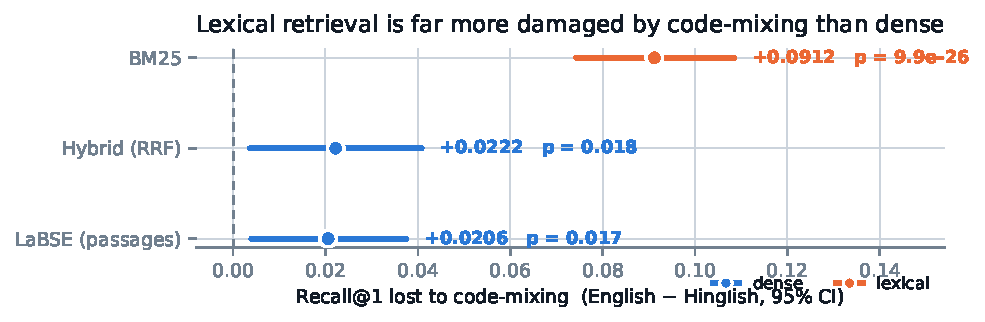
\includegraphics[width=0.9\textwidth]{figures/fig2_penalty.pdf}
\caption{Recall@1 lost to code-mixing, by retrieval system, with 95\% bootstrap
intervals. Lexical retrieval is far more damaged than dense.}\label{fig:penalty}
\end{figure}

\paragraph{Script, not language.} On the single-vector index, MuRIL --- pretrained on
Indian languages --- performs at the random floor for Hinglish ($0.0640$ versus a floor
of $0.0626$) but recovers to $0.1821$ on the same content rendered in English. MuRIL is
trained on Devanagari Hindi whereas MMCQSD is romanised. The failure is therefore one of
\emph{script} rather than of language, which has direct consequences for encoder
selection in code-mixed settings.

\subsection{The metric does not discriminate}\label{subsec:res-metric}

Scored against the unbiased reference, a constant answer consisting of the single word
\emph{``swelling''} attains a concept precision of $0.7132$. The grounded system attains
$0.1528$. A hard-coded word outperforms the real system by a factor of $4.7$.

The cause is structural: precision alone rewards asserting few concepts. Absolute levels
of this metric therefore carry no information about answer quality, and only paired
differences between arms scored identically are interpretable. We report $F_1$
throughout and ship the constant-answer rows with every table. We further note that the
commonly-reported ``hallucination rate'' is, under this definition, exactly
$1 - \mathrm{precision}$, so reporting both double-counts a single result.

\subsection{Grounding depends on the reference}\label{subsec:res-grounding}

Table~\ref{tab:grounding} scores the \emph{same} generations against both references.

\begin{table}[htbp]
\caption{Grounding effect on concept $F_1$ (grounded minus zero-shot), by reference.
Benjamini--Hochberg corrected.}\label{tab:grounding}
\begin{tabular}{@{}llcc@{}}
\toprule
Generator & Evidence & Circular ref. & Unbiased ref. \\
\midrule
llama-3.1-8b  & oracle          & $+0.203$ & $+0.062$ \\
gpt-oss-120b  & oracle          & $+0.093$ & $-0.021$\,(n.s.) \\
gpt-oss-120b  & real retrieval  & $-0.032$\,(n.s.) & $\mathbf{-0.047}$ \\
\botrule
\end{tabular}
\end{table}

Under the circular reference, grounding appears strongly beneficial. Under a reference
neither arm saw, the effect shrinks by a factor of three on one generator and becomes
significantly \emph{negative} on the other. The mechanism is visible in the components:
grounding raises precision and lowers recall (oracle arm, unbiased reference:
$-0.1384$ recall, BH $p = 0.00025$). Grounding makes the model more conservative, and
whether that trade is profitable depends on the generator.
Figure~\ref{fig:reference} shows all six contrasts with intervals.

\begin{figure}[htbp]
\centering
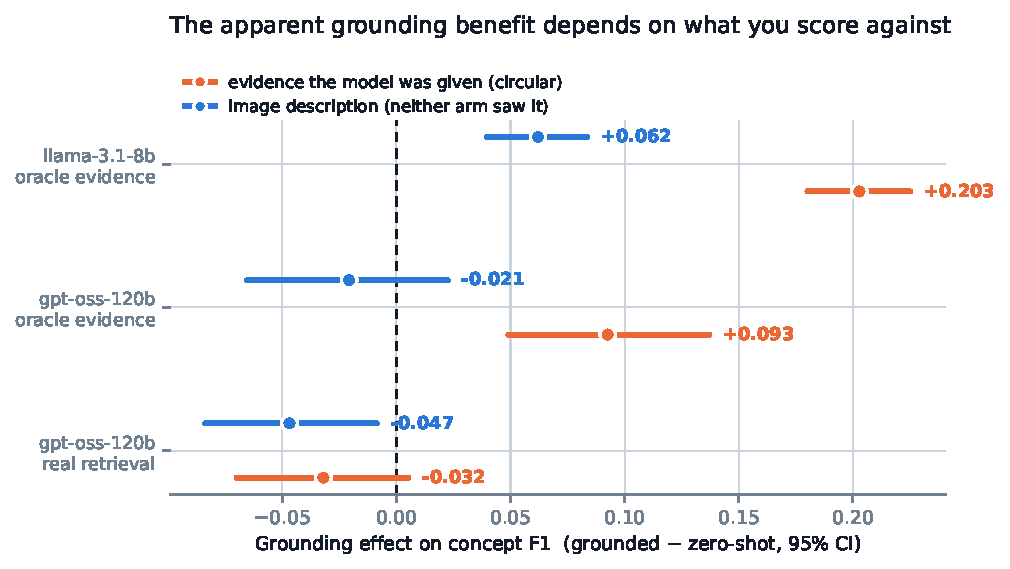
\includegraphics[width=0.9\textwidth]{figures/fig3_h1_reference_effect.pdf}
\caption{The same generations scored against two references give opposite
answers.}\label{fig:reference}
\end{figure}

\paragraph{Refusal is a first-class outcome.} With real retrieval the grounded arm
declines to answer in 33.8\% of cases (zero-shot: 0.2\%), typically stating that the
evidence concerns a different patient. Refusals assert no clinical concept and therefore
score as missing, disappearing from a naive mean --- which would make the system appear
healthiest exactly where it fails. We report answer coverage (49--52\% for grounded
arms, 92.9\% zero-shot) alongside every factuality figure.

\subsection{Code-mixing intensity, and two negative results}\label{subsec:res-ablation}

\paragraph{H\textsubscript{2}: intensity.} Using a repaired code-mixing measure, grounded
factual support is flat with respect to code-mixing intensity ($\rho = -0.0006$,
$p = 0.98$) while the zero-shot arm degrades significantly ($\rho = -0.116$, BH
$p = 0.0003$). Grounding absorbs the degradation that code-mixing induces in the
ungrounded model. We note that the measure required repair: the original lexicon
counted the English words \emph{doctor} and \emph{please} as Hindi, and they occur in
68.2\% and 35.7\% of queries respectively.

\paragraph{Adaptive truncation does not transfer.} A published similarity-gap heuristic
for adaptive context selection fires on $0$ of $3{,}015$ queries at its specified
threshold: it requires a $0.248$ similarity gap between adjacent neighbours, and the
largest gap occurring anywhere in the data is $0.109$. Swept across thresholds and
compared against a fixed $k$ at matched evidence budget, it wins $0$ of $6$ settings.
Precision is flat ($0.112$--$0.115$) at every setting while recall falls monotonically,
indicating that the similarity gap carries no relevance information here.

\paragraph{A configuration defect dominated the retrieval comparison.} The index was
originally built with a sequence limit of 128 tokens, truncating 100\% of case
narratives (median 307 tokens) and 52.5\% of queries, while lexical baselines read the
full document. Correcting this and adding passage chunking moved dense Recall@1 on
Hinglish from $0.1144$ to $0.1280$ and reversed the ordering against BM25. We report
this because the uncorrected comparison would have supported the opposite conclusion.

%% =====================================================================
\section{Discussion}\label{sec:discussion}

The results support a single claim: for code-mixed clinical RAG, \emph{measurement
design currently dominates architecture} in determining reported gains. The same
generations yield $+0.203$ or $-0.047$ concept $F_1$ depending only on the reference
text; a one-word constant answer outscores the system by $4.7\times$ on the standard
metric; and the most-cited comparison in our own Table~\ref{tab:retrieval} reversed once
a sequence-limit defect was corrected.

The retrieval findings are more robust and more actionable. The $4.4\times$ asymmetry
between lexical and dense degradation is a direct empirical argument for cross-lingual
embedding in code-mixed settings, and the MuRIL result refines it: what matters is
script coverage, not nominal language coverage. Practitioners deploying
Indian-language encoders on romanised user text should expect near-chance retrieval.

\subsection{Limitations and Threats to Validity}\label{subsec:limitations}

\begin{itemize}
\item \textbf{Relevance labels are coarse.} Condition-group matching over 18 groups
admits cases that are same-group but clinically irrelevant. Absolute Recall values
should be read as a lower bound.
\item \textbf{The concept lexicon is not clinician-validated} and covers 26 concepts.
It cannot capture findings outside that vocabulary.
\item \textbf{The unbiased reference is narrow and repetitive.} The image description
averages 1.5 concepts and takes 412 distinct values over 2,988 rows; we address the
non-independence with cluster bootstraps but the construct remains partial.
\item \textbf{Generator dependence.} Two of our generation results differ in sign
between generators. We report both rather than selecting one.
\item \textbf{Provider instability.} A model central to the study was withdrawn during
it.
\item \textbf{H\textsubscript{3} was not run.} Evidence-provenance comparison was cut:
PubMedQA is only 2.1\% on-topic for these conditions and MMedBench is 57.6\%
non-English, so the comparison would have measured corpus topicality rather than
provenance.
\item \textbf{No clinical deployment claim is made.} Absolute Recall@1 of $0.175$ is far
below what patient-facing use would require.
\end{itemize}

%% =====================================================================
\section{Conclusion and Future Work}\label{sec:conclusion}

We measured a Hinglish clinical RAG pipeline and found that code-mixing imposes a
significant retrieval penalty which is four times larger for lexical than for dense
retrieval; that an Indian-language encoder fails on romanised text for reasons of
script rather than language; and that the apparent factuality benefit of grounding is
substantially an artefact of scoring answers against the evidence they were conditioned
on. We release the corrected evaluation, the degenerate baselines that expose the
metric's failure mode, and two negative results.

Future work should establish a random-evidence control to separate genuine grounding
from evidence echoing, validate the concept lexicon against clinician annotation, and
extend the analysis to the multimodal signal that MMCQSD provides but that this
text-only study does not use.

%% =====================================================================
\bmhead{Supplementary Information}

%% TODO: confirm what is submitted alongside the manuscript.

\bmhead{Acknowledgements}

%% TODO: acknowledge supervisors and institutional support.

\section*{Declarations}

\textbf{Funding}\quad The authors received no specific funding for this work.

\textbf{Competing interests}\quad The authors declare no competing interests.

\textbf{Ethics approval and consent to participate}\quad Not applicable. All corpora
are publicly available and de-identified.

\textbf{Consent for publication}\quad Not applicable.

\textbf{Data availability}\quad MMCQSD and MultiCaRe are publicly available.
%% TODO: mint a Zenodo DOI for the derived pair file, index and result CSVs.
Derived artefacts and all result files are archived at %% TODO: DOI.

\textbf{Materials availability}\quad Not applicable.

\textbf{Code availability}\quad All source code, prompts, configuration and analysis
scripts are available at %% TODO: repository URL and release tag.
A single entry point regenerates every reported number and figure from cached
artefacts.

\textbf{Author contributions}\quad %% TODO: complete per CRediT roles.

\bibliography{ICCSDI2026-references}

\end{document}
